\documentclass[sigconf,nonacm]{acmart}
\usepackage[frozencache=true]{minted}
\usepackage{tikz} % for figures
\usetikzlibrary{arrows.meta,shapes.geometric}

\hyphenation{time-stamp time-stamps re-con-cilia-tion data-center}

\begin{document}
\title{TODO: Title}
\subtitle{Keynote at the 15th ACM International Conference on Distributed and Event-Based Systems}

\author{Martin Kleppmann}
\orcid{0000-0001-7252-6958}
\affiliation{%
  \institution{University of Cambridge}
  \city{Cambridge}
  \country{UK}
}
\email{mk428@cst.cam.ac.uk}

\begin{abstract}
TODO: Abstract
\end{abstract}

\begin{CCSXML}
<ccs2012>
  <concept>
    <concept_id>10002951.10002952.10002953.10010820.10003208</concept_id>
    <concept_desc>Information systems~Data streams</concept_desc>
    <concept_significance>500</concept_significance>
  </concept>
  <concept>
    <concept_id>10011007.10010940.10010971.10010972.10010975</concept_id>
    <concept_desc>Software and its engineering~Publish-subscribe / event-based architectures</concept_desc>
    <concept_significance>500</concept_significance>
  </concept>
  <concept>
    <concept_id>10010405.10010406.10010422</concept_id>
    <concept_desc>Applied computing~Event-driven architectures</concept_desc>
    <concept_significance>300</concept_significance>
  </concept>
  <concept>
    <concept_id>10003752.10003753.10003761.10003763</concept_id>
    <concept_desc>Theory of computation~Distributed computing models</concept_desc>
    <concept_significance>300</concept_significance>
  </concept>
</ccs2012>
\end{CCSXML}

\ccsdesc[500]{Information systems~Data streams}
\ccsdesc[500]{Software and its engineering~Publish-subscribe / event-based architectures}
\ccsdesc[300]{Applied computing~Event-driven architectures}
\ccsdesc[300]{Theory of computation~Distributed computing models}

\keywords{stream processing, event sourcing, CRDTs, state machine replication}
\maketitle

% Title: Event-based thinking in collaboration software

% What do Google Docs and stream processing have in common? Both are centered around the idea of streams of events. In the case of Google Docs and other collaboration software, each event describes a change that a user has made to a document. Each user's local device has a copy of the shared document, and processing the stream of changes means updating this local copy so that it is consistent with all of the other users' copies of the document.

% This talk will explore collaboration software through the lens of event-based thinking, explaining some of the algorithms that are used to implement this kind of software, such as Conflict-free Replicated Data Types (CRDTs). We will highlight new developments in this area, such as local-first software, and identify some open challenges in the area.

\section{Introduction}

\section{A Taxonomy of Event-based Systems}

The term \emph{event} is used in many different ways in different branches of computing.
Many authors talk about events without always being explicit about the precise context they are referring to.
In order to facilitate a precise discussion of the trade-offs, I present a taxonomy that categorises the different uses of events, based on the flowchart in \autoref{fig:flowchart}.
Such a broad-brush taxonomy cannot necessarily capture all of the nuance of the field, and sometimes the boundaries between categories can be blurry.
Nevertheless, I hope that it will be a useful tool for structuring discussions.

\begin{figure*}
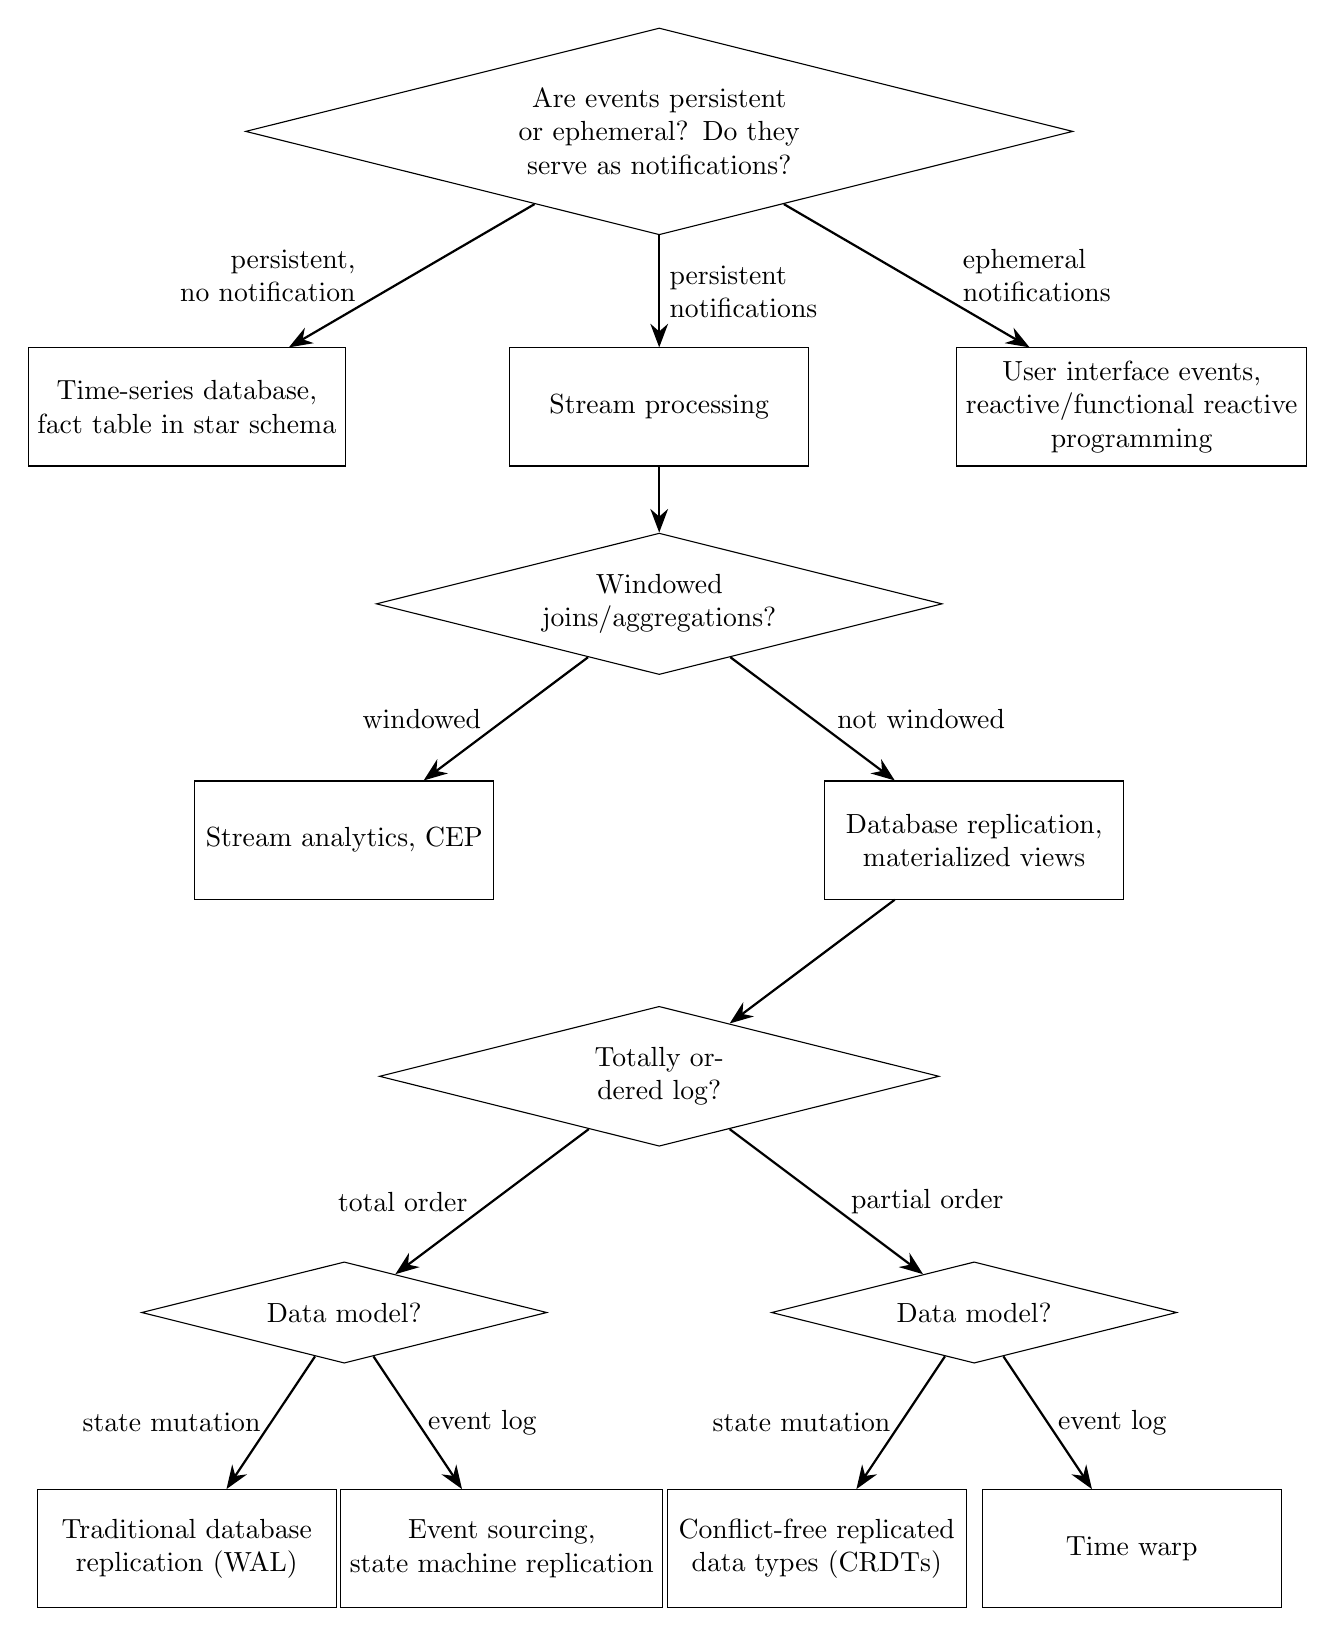
\begin{tikzpicture}
\tikzstyle{question}=[diamond,draw,aspect=4,text width=3cm,align=center]
\tikzstyle{box}=[rectangle,draw,align=center,minimum width=3.8cm,minimum height=1.5cm]
\tikzstyle{arrow}=[{Stealth[length=3mm]}-,thick]
\node [diamond,draw,text width=5cm,align=center,aspect=4] (n1) at (0,0) {Are events persistent or ephemeral? Do they serve as notifications?};
\node (n2) [box] at (-6,-3.5) {Time-series database,\\fact table in star schema} edge [arrow] node [left,align=right,inner xsep=7mm] {persistent,\\no notification} (n1);
\node (n3) [box] at (0,-3.5) {Stream processing} edge [arrow] node [right,align=left] {persistent\\notifications} (n1);
\node (n4) [box] at (6,-3.5) {User interface events,\\reactive/functional reactive\\programming} edge [arrow] node [right,align=left,inner xsep=7mm] {ephemeral\\notifications} (n1);
\node (n5) [question] at (0,-6) {Windowed joins/aggregations?} edge [arrow] (n3);
\node (n6) [box] at (-4,-9) {Stream analytics, CEP} edge [arrow] node [left,inner xsep=3mm] {windowed} (n5);
\node (n7) [box] at (4,-9) {Database replication,\\materialized views} edge [arrow] node [right,inner xsep=3mm] {not windowed} (n5);
\node (n8) [question] at (0,-12) {Totally ordered log?} edge [arrow] (n7);
\node (n9) [question] at (-4,-15) {Data model?} edge [arrow] node [left,inner xsep=3mm] {total order} (n8);
\node (n10) [box] at (-6,-18) {Traditional database\\replication (WAL)} edge [arrow] node [left] {state mutation} (n9);
\node (n11) [box] at (-2,-18) {Event sourcing,\\state machine replication} edge [arrow] node [right] {event log} (n9);
\node (n12) [question] at (4,-15) {Data model?} edge [arrow] node [right,inner xsep=3mm] {partial order} (n8);
\node (n13) [box] at (2,-18) {Conflict-free replicated\\data types (CRDTs)} edge [arrow] node [left] {state mutation} (n12);
\node (n14) [box] at (6,-18) {Time warp} edge [arrow] node [right] {event log} (n12);
\end{tikzpicture}
\centering
\caption{A taxonomy of event-based systems.}
\label{fig:flowchart}
\end{figure*}

\subsection{Notifications and persistence}

At a high level, an event can be:
\begin{itemize}
\item a notification about the fact that something happened;
\item a persistent record of the fact that something happened; or
\item both.
\end{itemize}

Examples of notification events occur in many applications.
JavaScript code running in a web browser can register functions to be called when the user does something, such as clicking or typing a key on the keyboard: here the click or the key-press is the event.
Most other user interface frameworks have a similar system of dispatching user input events to callback functions or \emph{event handlers}.
Many operating systems offer asynchronous (non-blocking) I/O functionality, in which case a thread runs an \emph{event loop} that processes notifications from the OS when requested I/O operations complete.
Reactive and functional reactive programming (FRP) offer higher-level APIs, such as a dataflow programming model, for working with \emph{streams of events}.
In all of these examples, an event is something that exists only in-memory in a single process; it is ephemeral, not persistent, in the sense that it is not normally written to disk.
Ephemeral events exist only for the lifetime of a process and are not preserved across restarts.

In contrast, persistent events do not necessarily have a notification element.
For example, time-series databases are often used to record events that occurred over time, such as periodic readings from a sensor, price updates of a financial asset, and tracking the activity of a person or machine.
Another example is the fact table that appears in the star or snowflake schema of data warehouses and business analytics systems: every row in the fact table is typically a timestamped record of an event that happened, such as the purchase of a particular product by a particular customer.
In such systems, an event is a value that is recorded in a database for future analysis, but the receipt of the event does not necessarily trigger the immediate execution of any application code.
The primary purpose of the events from the user's point of view is to allow the retroactive querying and analysis of the event history, such as examining trends and generating reports showing the change of some metric over time.

Some systems combine these characteristics such that an event is both a persistent record of the fact that something happened, and also a notification (i.e.\ application code is called to handle the occurrence of an event).
I will broadly group such systems under the term \emph{stream processing}, and break them down into subcategories later.
Some databases provide facilities such as \emph{materialized view maintenance} and \emph{continuous queries} (queries whose results are automatically updated as the underlying data changes), which can also be regarded as a form of notification.

Many programming models for distributed systems are based on sending and receiving messages, and the receipt of a message can also be seen as a notification event that triggers the execution of application code.
For example, the \emph{actor model} is a widely-used approach in which multiple actors or lightweight threads, potentially located on different machines, communicate by sending each other messages.
In many actor systems these messages are ephemeral (they might be lost if a part of the system crashes or if the network is unreliable), but some actor frameworks also include persistence mechanisms for actor state and/or the messaging middleware.
For the purposes of this taxonomy I will reserve the term ``persistent'' for those systems in which message delivery is reliable, data is durable, and all state in the system is preserved in case of a crash or network fault; any systems with best-effort message delivery fall into the ``ephemeral notifications'' category.

\subsection{Windowing in stream processing}\label{sec:windowing}

Zooming in on the systems that provide both persistence and notifications, we can further differentiate them by examining the kind of logic that can be performed in response to an event.
The very simplest stream processors use stateless operators, in which every event can be processed independently of any other event, based only on the information in that event (for example, selecting events where a certain property of the event falls within some set of values).
Most interesting applications also require event processing logic that combines information from several events: in database parlance, a \emph{join} or \emph{grouping} of events.
Events may be combined by aggregation (e.g.\ computing the count, sum, or average of some property of a set of events), by emitting compound events that include properties from several input events, or by more complex state machines that we discuss in \autoref{sec:smr}.

Some stream processing systems are designed primarily for applications in which the events that need to be combined occur fairly close together in time.
For example, a stock trading system may need to compute the minimum and maximum prices of an asset per hour or per day, or a fraud detection system may need to detect unusual patterns of recent activity on a customer's credit card.
Such operations are known as \emph{windowed} joins or aggregations.
Several types of window are in use (such as tumbling or sliding windows), but they all have in common that they place a bound on the maximum time interval between any two events that may be combined; any events that are further apart in time than this bound are treated as unrelated.
Windowed processing often occurs when performing business analytics on streams, or in \emph{complex event processing} (CEP).

On the other hand, some applications need to combine events that may lie arbitrarily far apart in time, and thus windowing is not applicable.
For example, imagine a Twitter-like social network in which users may post messages and update their profile photo.
Posting a message is one type of event, and updating the photo is another type of event.
Now say that for display purposes we want to attach the sender's most recent profile photo to every message-posting event.
It may well be that the user last updated their profile photo years ago, and thus, finding the current photo requires going back arbitrarily far in the stream of profile photo update events.

In a SQL database, this join between messages and profile photos might be expressed as follows:

\begin{minted}{sql}
SELECT messages.*, profiles.photo_url
FROM messages
JOIN profiles ON messages.sender_id = profiles.user_id
\end{minted}

The message-posting event in an event-based system corresponds to inserting a row into this \texttt{messages} table, and the photo-updating event corresponds to updating the user's entry in the \texttt{profiles} table.
A stream processor that combines these events is effectively acting as a continuous query execution engine that maintains the output of the query above, i.e.\ maintaining a materialised view of the query.
It may perform the join using a database that contains the most recent profile photo per user, updating that database on every photo-updating event, and querying that database on every message-posting event.

One detail that such a system needs to decide is: when a user updates their profile photo, do we go back and retroactively attach the most recent photo to all of the user's past messages, or do we attach the new profile photo only to messages posted after the photo change?
The query above seems to suggest the former, and this is also what Twitter does in practice, but this means that the stream processor needs to be able to scan over the entire history of past message-posting events when a photo-updating event is received.
The latter policy might also be reasonable: it would be easier to implement in imperative code, but more complicated to express in SQL.

\subsection{Database replication and events}\label{sec:replication}

If we focus our attention on systems where the events are persistent notifications without windowing, we may notice a strong similarity to replication in database systems.
The goal of replication is to have a copy of the same data on several different machines: that is, any two replicas converge to the same state, and all committed transactions are reflected in that state.
Viewed through the lens of event-based systems, we can treat every transaction that modifies the database as an update event, the execution of an update (i.e.\ reflecting the update in the database state) as the processing of that event, and the replication of data from one machine to another as the propagation of that event through the distributed system.
Read-only transactions may or may not correspond to events, depending on the system.

In such a database system, the replication infrastructure ensures that every event corresponding to a committed transaction is eventually processed by every non-faulty replica.
We can classify such replication systems into two broad categories: those that arrange the replication events into a log, and those that use some other replication mechanism (such as gossip protocols, anti-entropy, or clients independently updating several replicas).
The key properties of a log are that the events in it are totally ordered (i.e.\ all replicas observe the log entries in the same order), and it is append-only (i.e.\ if a replica observes log entry A immediately followed by log entry B, then there will never be a log entry C that appears between A and B in the total order).

This append-only log is constructed either using a consensus protocol such as Raft or Multi-Paxos, or by designating one replica as the \emph{leader} (also known as master or primary) and all other replicas as followers (aka slaves or secondary).
In fact, most consensus protocols are essentially leader-based replication combined with an automatic mechanism for electing a new leader if the current leader fails.
The leader decides on the order in which events should be appended to the log, and all other replicas process the events in the order decided by the leader.

In many databases, the exact structure and content of the events in the log has traditionally been an implementation detail of the database system that is not exposed to applications.
For example, several database systems use the \emph{write-ahead log} (WAL) for replication, which consists of records indicating how the database's on-disk data structures are changing; others use a separate replication log.
More recently, \emph{change data capture} techniques have been developed to extract the data change events (rows inserted, updated, or deleted) from this log and make them available to applications via stream processing systems.

\subsection{State machine replication (SMR)}\label{sec:smr}

In WAL-based replication and change data capture, the primary data model used by the application is the database state that can be mutated by the application (e.g.\ by inserting, updating, or deleting rows in tables), and the data change events are generated automatically as a side-effect of these mutations.
It is also possible to swap these roles, making the data change events the primary data model of the application, so that any state changes become a side-effect of processing those events.
This is the idea behind \emph{state machine replication}~\cite{Schneider:1990}, and the closely related concept of \emph{event sourcing}~\cite{Fowler:2005}.

In state machine replication (SMR) and event sourcing, the application does not directly mutate the state of a database.
Instead, the application defines a set of event types that may occur, and whenever something happens, an event of the appropriate type is appended to an event log.
All replicas subscribe to this event log, and each replica processes events in the order in which they appear in the log.
The event processing function can use arbitrary logic to update the database state, as long as it is deterministic and it depends only on the current database state and the content of the event.
Provided that each replica processes the same sequence of events in the same order, and each replica starts in the same initial state (e.g.\ an empty database), the deterministic event processing logic ensures that all replicas end up in the same final state.
We can think of each replica as a state machine whose state is its copy of the database, and whose state transition function is the event processing function.
Put another way, the database state is a materialised view into the underlying event log.

An advantage of this approach is that well-designed events often capture the intent and meaning of operations better than events that are a mere side-effect of a state mutation.
For example, ``student $x$ cancelled their enrollment in course $y$ for reason $z$'' is a clear descriptive event, whereas ``one row was deleted from the \verb+enrollments+ table, one row was added to the \verb+cancellation_reasons+ table, and the \verb+available_places+ field of a course was incremented'' is a much less clear description that embeds a lot of irrelevant detail about the current database schema.
An event log thus makes it easier for the people who work with a system to understand how it got into a particular state, which can help with audit and debugging.

Another advantage of an event log is that it can be replayed in order to rebuild the resulting database state.
If the application developers wish to change the logic for processing an event, for example to change the resulting database schema or to fix a bug, they can set up a new replica, replay the existing event log using the new processing function, and then switch clients to reading from the new replica instead of the old one.
This sort of retroactive change in business logic is not usually possible in state-mutation databases.
It is easy to maintain several different views onto the same underlying event log if needed.
As long as the rate of updates is not too high, it is often feasible to retain the event log indefinitely and replay it occasionally as needed.

Blockchains and distributed ledgers also use SMR, in which case the chain of blocks (and the transactions therein) constitutes the event log, the ledger (e.g.\ the balance of every account) is the resulting state, and smart contracts or built-in transaction processing logic are the state transition function.

The downside of the event sourcing/SMR approach is that it is less familiar to most application developers than mutable-state databases, and the level of indirection between the event log and the resulting database state adds complexity in some types of applications that are more easily expressed in terms of state mutations.

\subsection{Events with a partial order}

Both WAL-based replication and SMR depend crucially on the assumptions that all replicas process events in exactly the same order.
Within a single datacenter, this is a reasonable assumption, since leader-based replication and consensus protocols work well in this setting.
However, if replicas are distributed across multiple geographic locations, or if the network between replicas is unreliable, constructing a log becomes expensive, since appending an event to the log requires at waiting least one network round-trip to the leader and/or a quorum of replicas.
In the extreme case, if we want a replica to be able to generate and process events even while it is completely disconnected from all other replicas (a system that is ``available'' and ``partition-tolerant'' in the sense of the CAP theorem~\cite{Gilbert:2002}), the assumption of a totally ordered log becomes impossible to satisfy.

In a system that allows disconnected operation it is still possible to enforce a total order for events; however, those events do not necessarily form a log because the structure is not append-only.

% TODO: figure showing how timestamps from different replicas get interleaved

CRDTs~\cite{Shapiro:2011}

virtual time~\cite{Jefferson:1985}

\bibliographystyle{ACM-Reference-Format}
\bibliography{references}{}

\end{document}
